%!TEX root = ../main.tex
\chapter{Estimation of the uncertainty of the time calibration.}
\label{appendix:calib_error}

In this appendix, a small study of the uncertainty made on the calibration from TDC to nanoseconds is done. By simple calculation, the conversion is done is the following way:
\begin{equation*}
	\begin{split}
		\text{T} \: \text{[ns]} & = ( \text{TDC} - \text{Ped} ) * \text{slope} \\
		& = ( \text{TDC} - \text{Ped} ) * \frac{\text{A}}{(\text{Max} - \text{Ped})} \quad \text{with A = 3920 ns}
	\end{split}
\end{equation*}

To avoid correlations between the slope and the pedestal, the uncertainty is obtained by differentiating w.r.t Max and Ped. The uncertainty is then obtained via:
\begin{equation*}
	\partial t^2 = \left(\frac{\partial t}{\partial Ped}\right)^2 \times \sigma_{Ped}^2 + \left(\frac{\partial t}{\partial Max}\right)^2 \times \sigma_{Max}^2 + \left(\frac{\partial t}{\partial A}\right)^2 \times \sigma_{A}^2
\end{equation*}

Assuming that $\sigma_{A}$ is null, we get the following formula:
\begin{equation*}
	\partial t^2 = \frac{1}{(\text{Max} - \text{Ped})^2} \left[ \left( \frac{\text{A(TDC - Max)}}{(\text{Max} - \text{Ped})} \right)^2 \times \sigma_{Ped}^2 + \left( \frac{\text{A(TDC - Ped)}}{(\text{Max} - \text{Ped})} \right)^2 \times \sigma_{Max}^2 \right]
\end{equation*}

As one can expect, the formula is symmetric and should be minimum in the middle of the ramp as long as $\sigma_{Max}$ and $\sigma_{Ped}$ are similar. On the other hand, the uncertainty will be greater on one side or the other depending on the $\sigma$ being the biggest. The uncertainties estimations $\sigma_{Max}$ and $\sigma_{Ped}$ are described in subsection \ref{subsec:slope_calib}. Distributions of the uncertainties extracted can be seen in figures \ref{fig:error_ped} and \ref{fig:error_max}. Theses uncertainties are obtained arbitrary due to the threshold and maximum variation and are likely to be over-estimated as they are not reflected in the final timing distribution. Moreover, the shift of the distribution to zero is correcting any uncertainty made on the pedestal for each channels thus $\sigma_{Ped}$ is likely very small.

\begin{figure}[thtbp!]
	\begin{subfigure}[t]{0.49\textwidth}
		\centering
		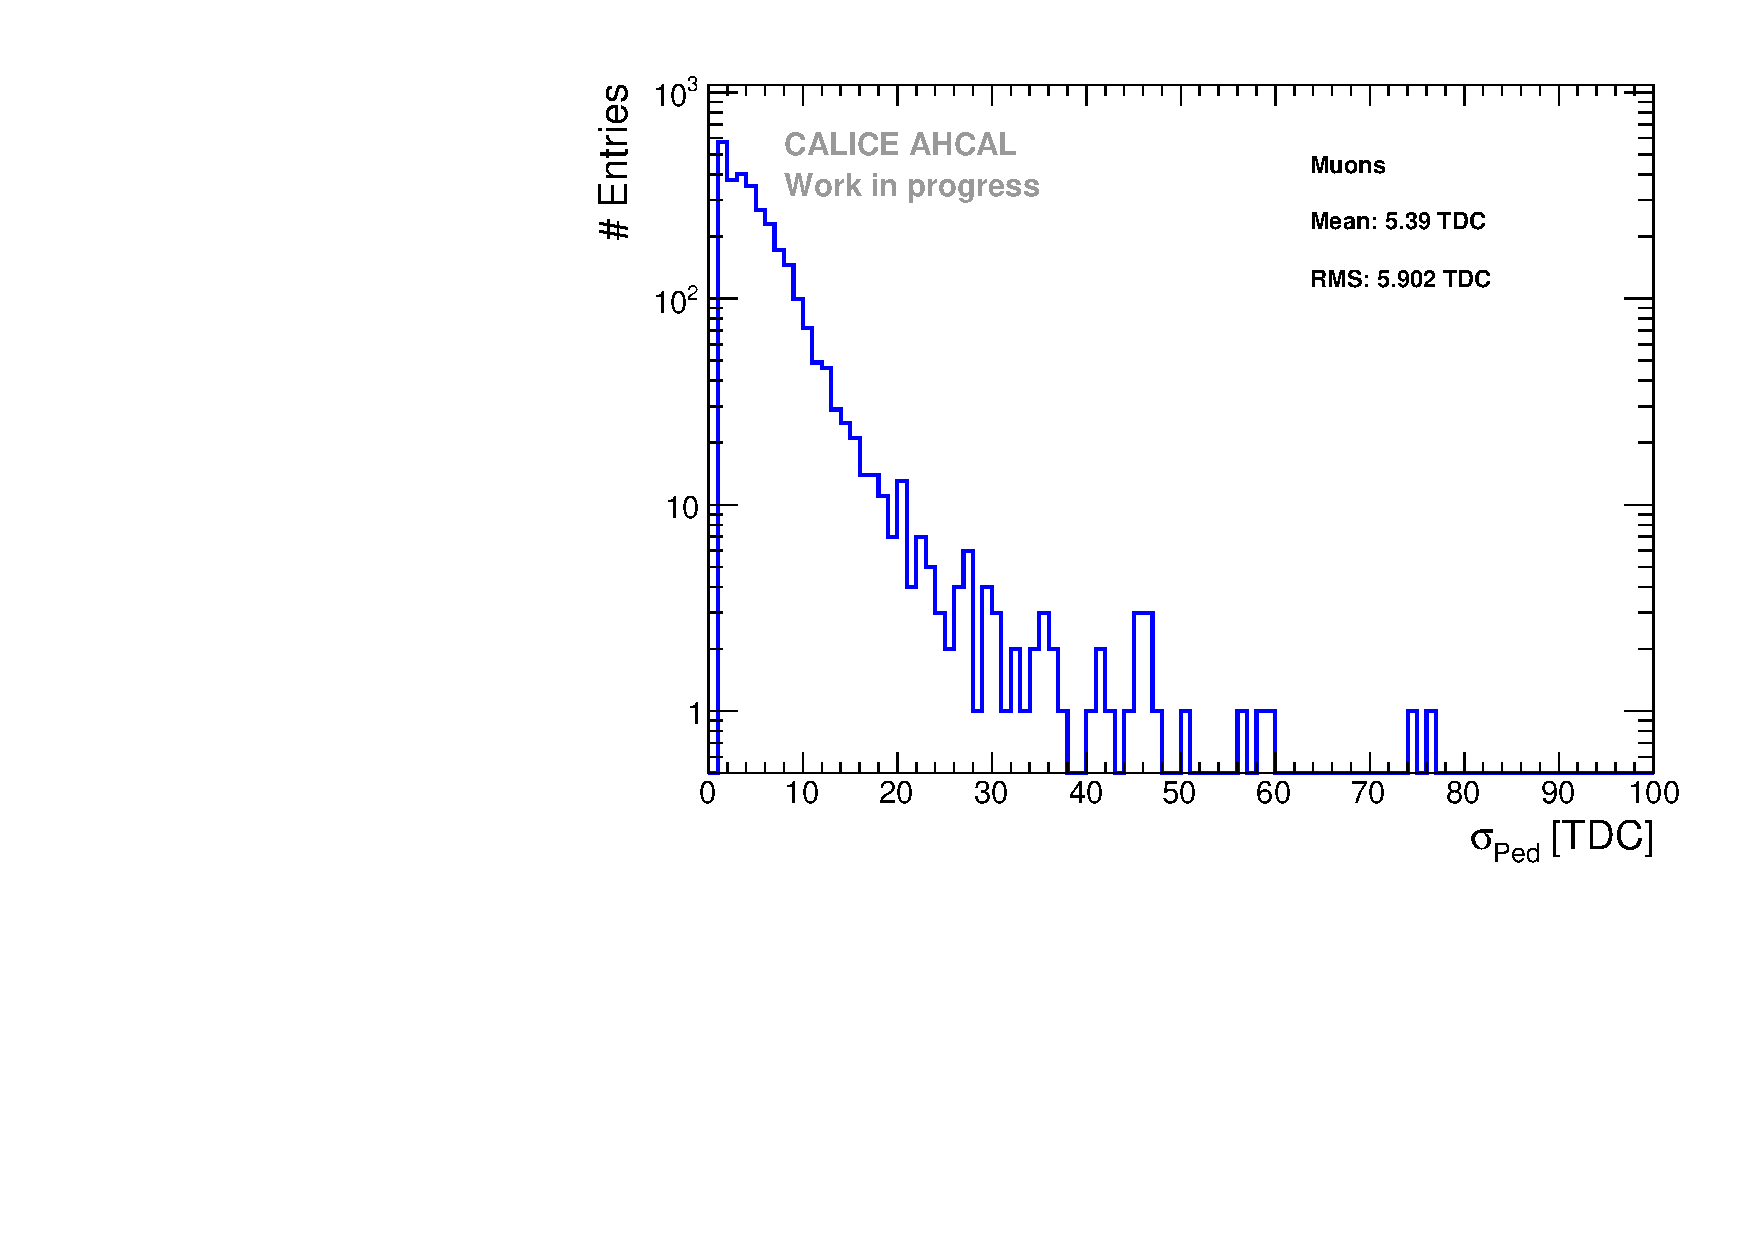
\includegraphics[width=1\linewidth]{../Thesis_Plots/Timing/Muons/Plots/PedestalErrorDistribution_AHCAL.pdf}
		\caption{Encertainties extracted from the edge detection for the pedestal for each chip. channel, memory-cell and BXID.} \label{fig:error_ped}
	\end{subfigure}
	\hfill
	\begin{subfigure}[t]{0.49\textwidth}
		\centering
		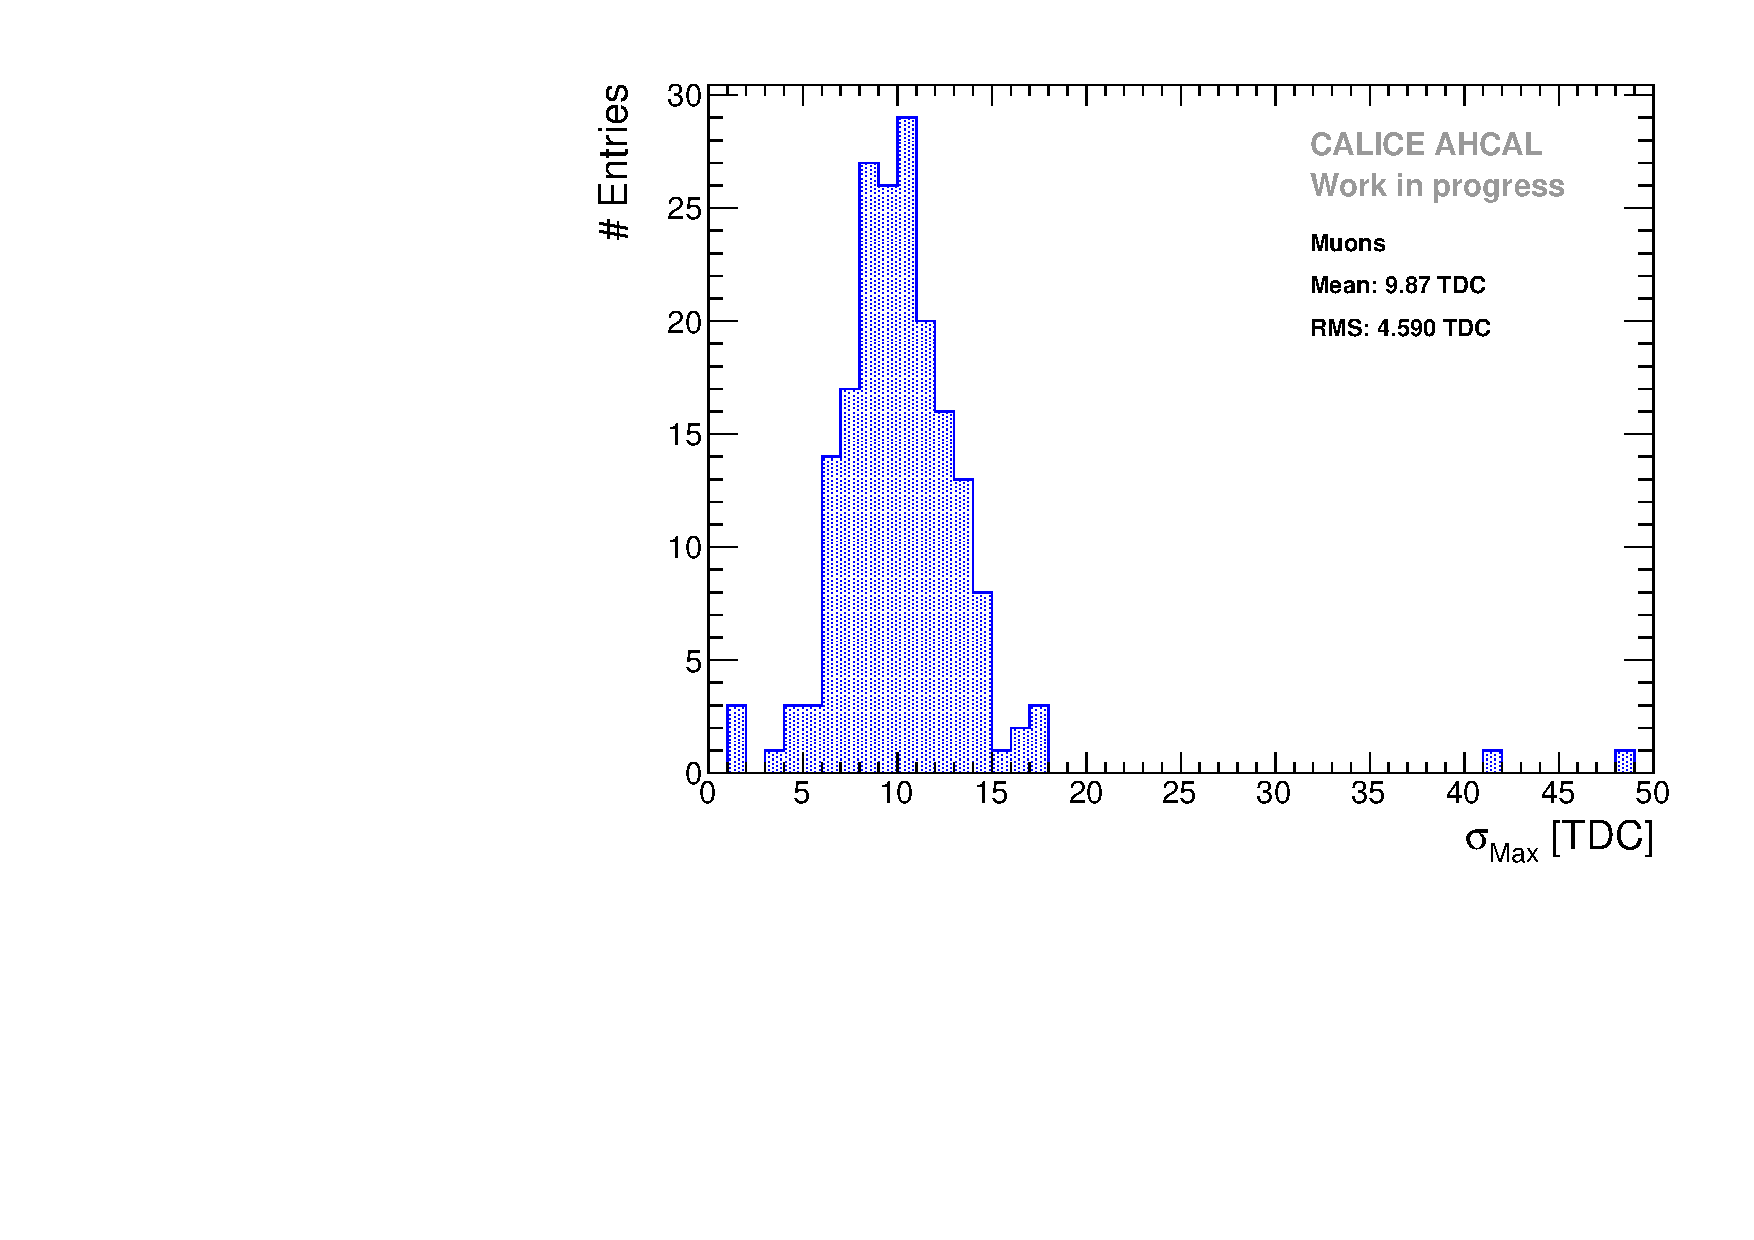
\includegraphics[width=1\linewidth]{../Thesis_Plots/Timing/Muons/Plots/MaxErrorDistribution_AHCAL.pdf}
		\caption{Uncertainty extracted from the edge detection for the maximum of the ramp for each chip and BXID.} \label{fig:error_max}
	\end{subfigure}
	\caption{\subref{fig:error_ped}) Pedestal uncertainty distribution extracted for all channels in the detector, most of the errors made are small with a high tail certainly due to the limited statistics for some channels. $\mu$ = 5.37 TDC, RMS = 5.82 TDC \subref{fig:error_max}) Maximum uncertainty distribution extracted from the edge detection method for each chip and BXID. The error is a bit higher than for the pedestal in general due to the difficulty to detect perfectly the end of the ramp. $\mu$ = 9.85 TDC, RMS = 4.60 TDC.}
\end{figure}

The figure \ref{fig:error_chn2} represent the uncertainty made for one channel selected in a single chip for a single memory cell and BXID. It shows the symmetric behavior of the error and present a minimum around the middle of the ramp. This not a typical channel as mostly the maximum has an error higher than the pedestal due to the difficulty to pick perfectly the maximum of the ramp with the sharp falling edge. A more typical channel can be seen in figure \ref{fig:error_chn}.

\begin{figure}[htbp!]
	\begin{subfigure}[t]{0.49\textwidth}
		\centering
		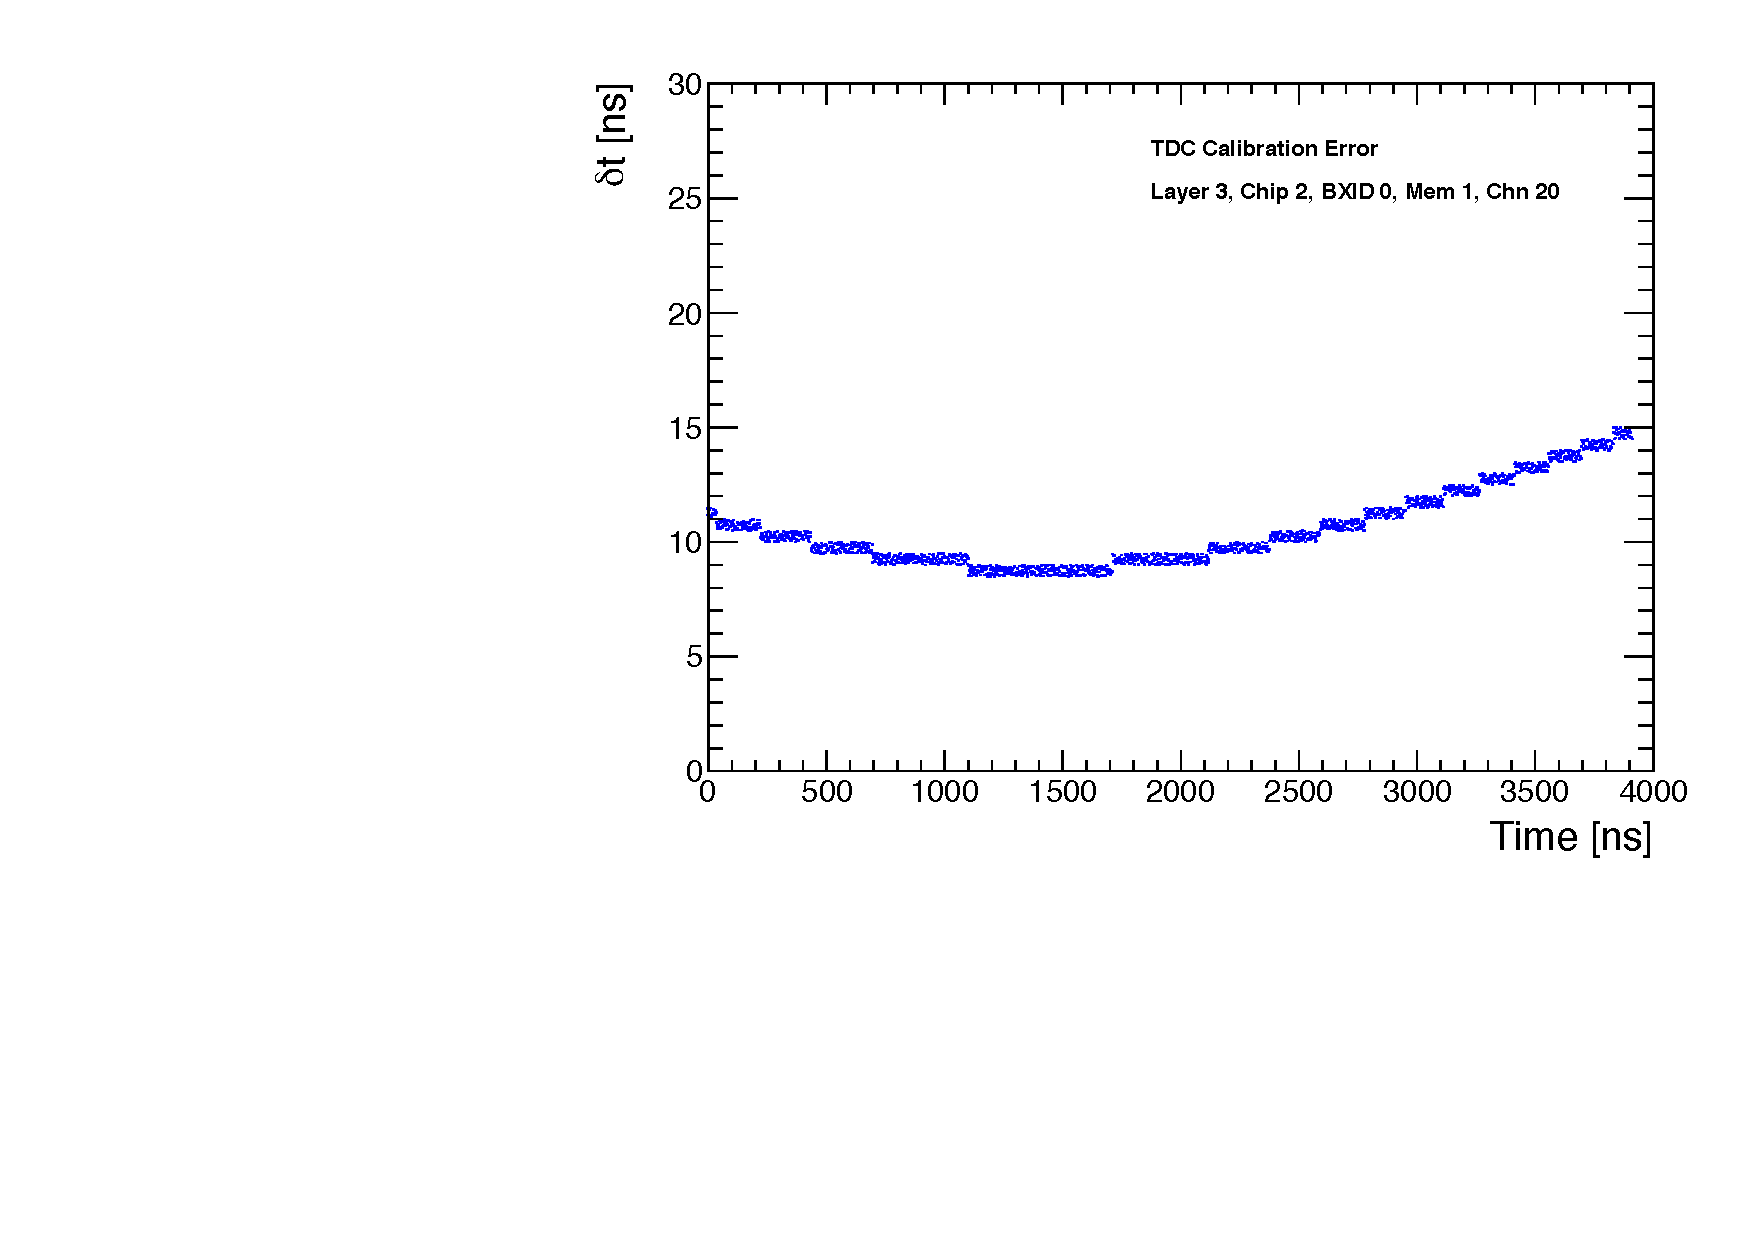
\includegraphics[width=1\linewidth]{../Thesis_Plots/Timing/Muons/Plots/TimeErrorEstimation_Layer3.pdf}
		\caption{Uncertainties extracted from the edge detection for the pedestal for each chip. channel, memory-cell and BXID.} \label{fig:error_chn}
	\end{subfigure}
	\hfill
	\begin{subfigure}[t]{0.49\textwidth}
		\centering
		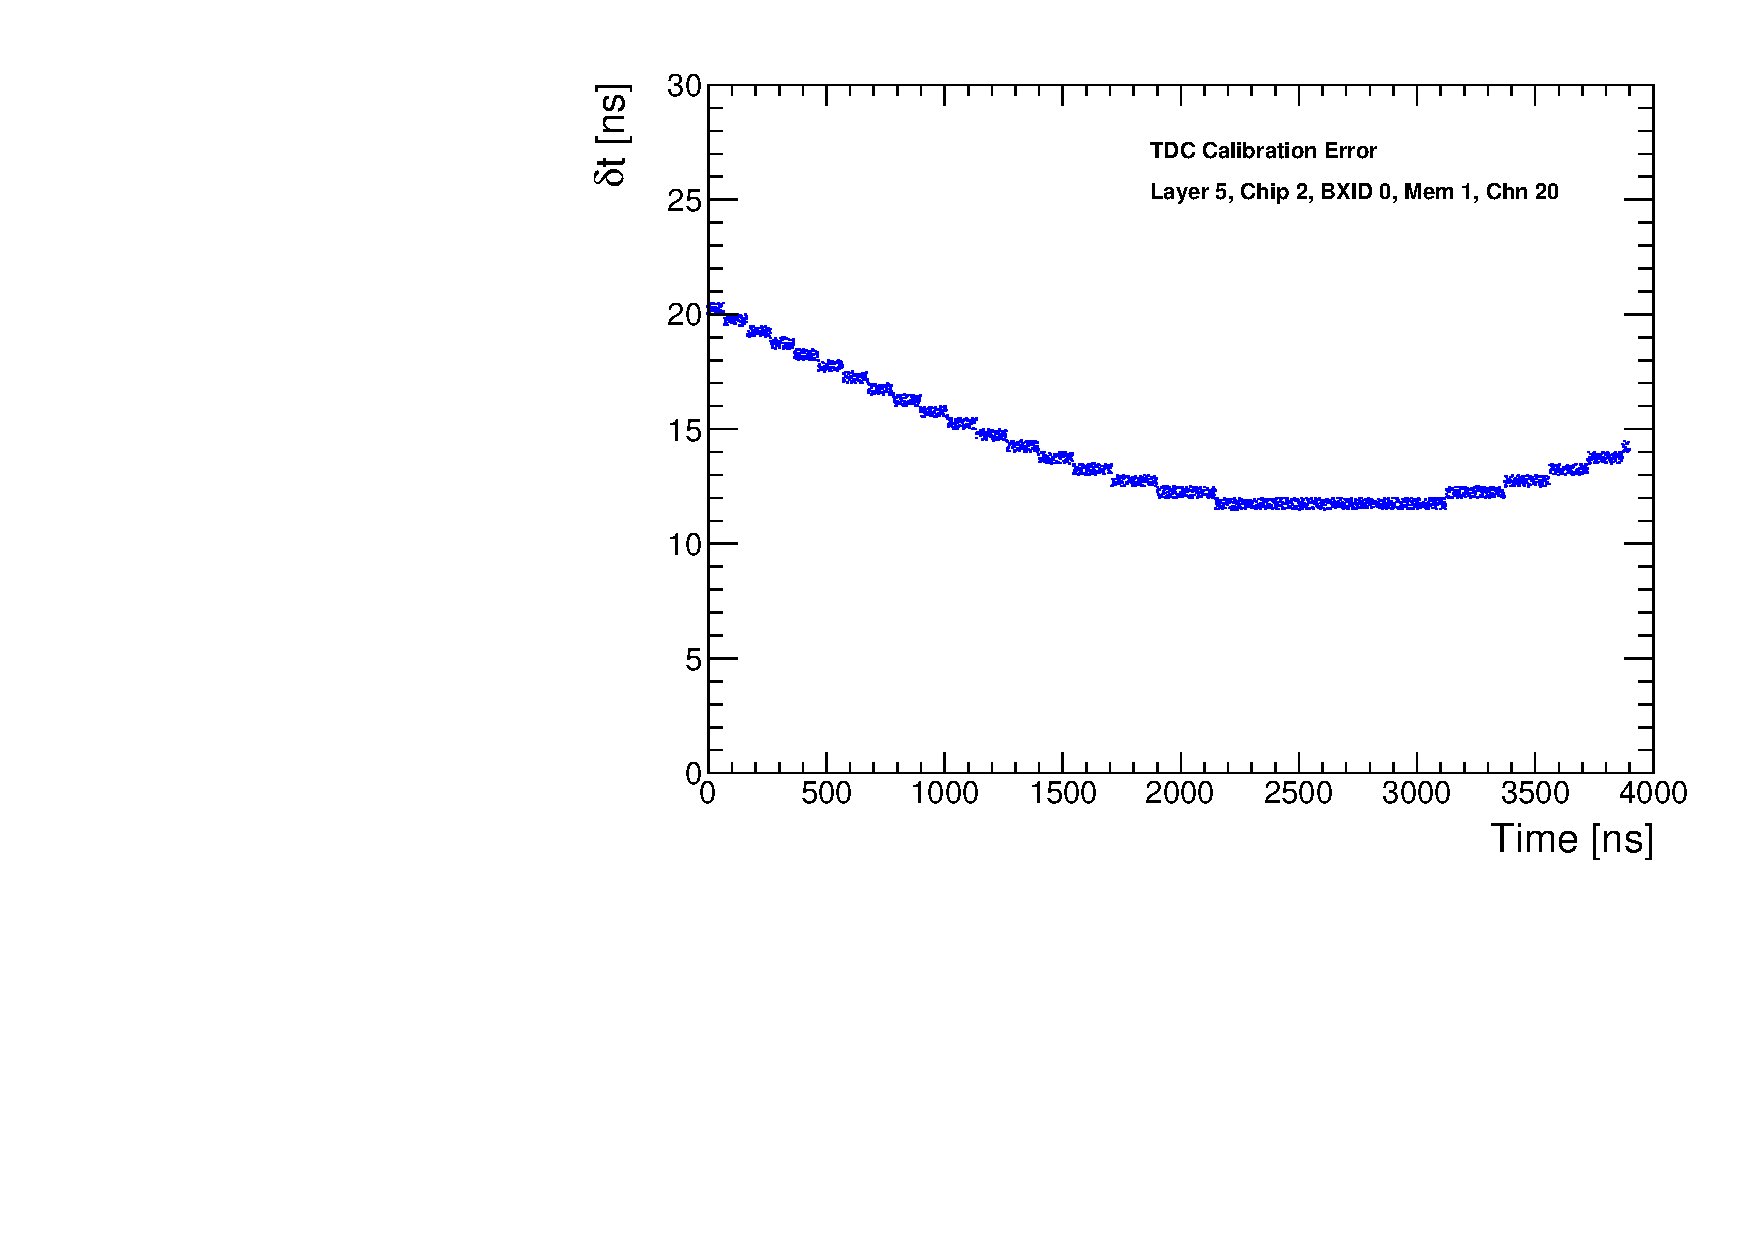
\includegraphics[width=1\linewidth]{../Thesis_Plots/Timing/Muons/Plots/TimeErrorEstimation_Layer5.pdf}
		\caption{Calibration uncertainty made on the conversion to nanosecond for a channel on layer 5.} \label{fig:error_chn2}
	\end{subfigure}
	\caption{\subref{fig:error_chn}) Uncertainty distribution made for a single channel on layer 3. The error is variating between 9 and 14 ns but is likely to be over-estimated and not valid for the final time distribution \subref{fig:error_chn2}) Uncertainty distribution made for a single channel on layer 5. The uncertainty is between 12 and 20 ns but is likely to be over-estimated and not valid for the final time distribution.}
\end{figure}
